\documentclass[border=10pt]{standalone}

\usepackage{tikz}
\usepackage{tikzsymbols}
\usetikzlibrary{calc,patterns,shapes.geometric}

\def\centerarc[#1](#2)(#3:#4:#5){\draw[#1] ($(#2)+({#5*cos(#3)},{#5*sin(#3)})$) arc (#3:#4:#5);}

\begin{document}
	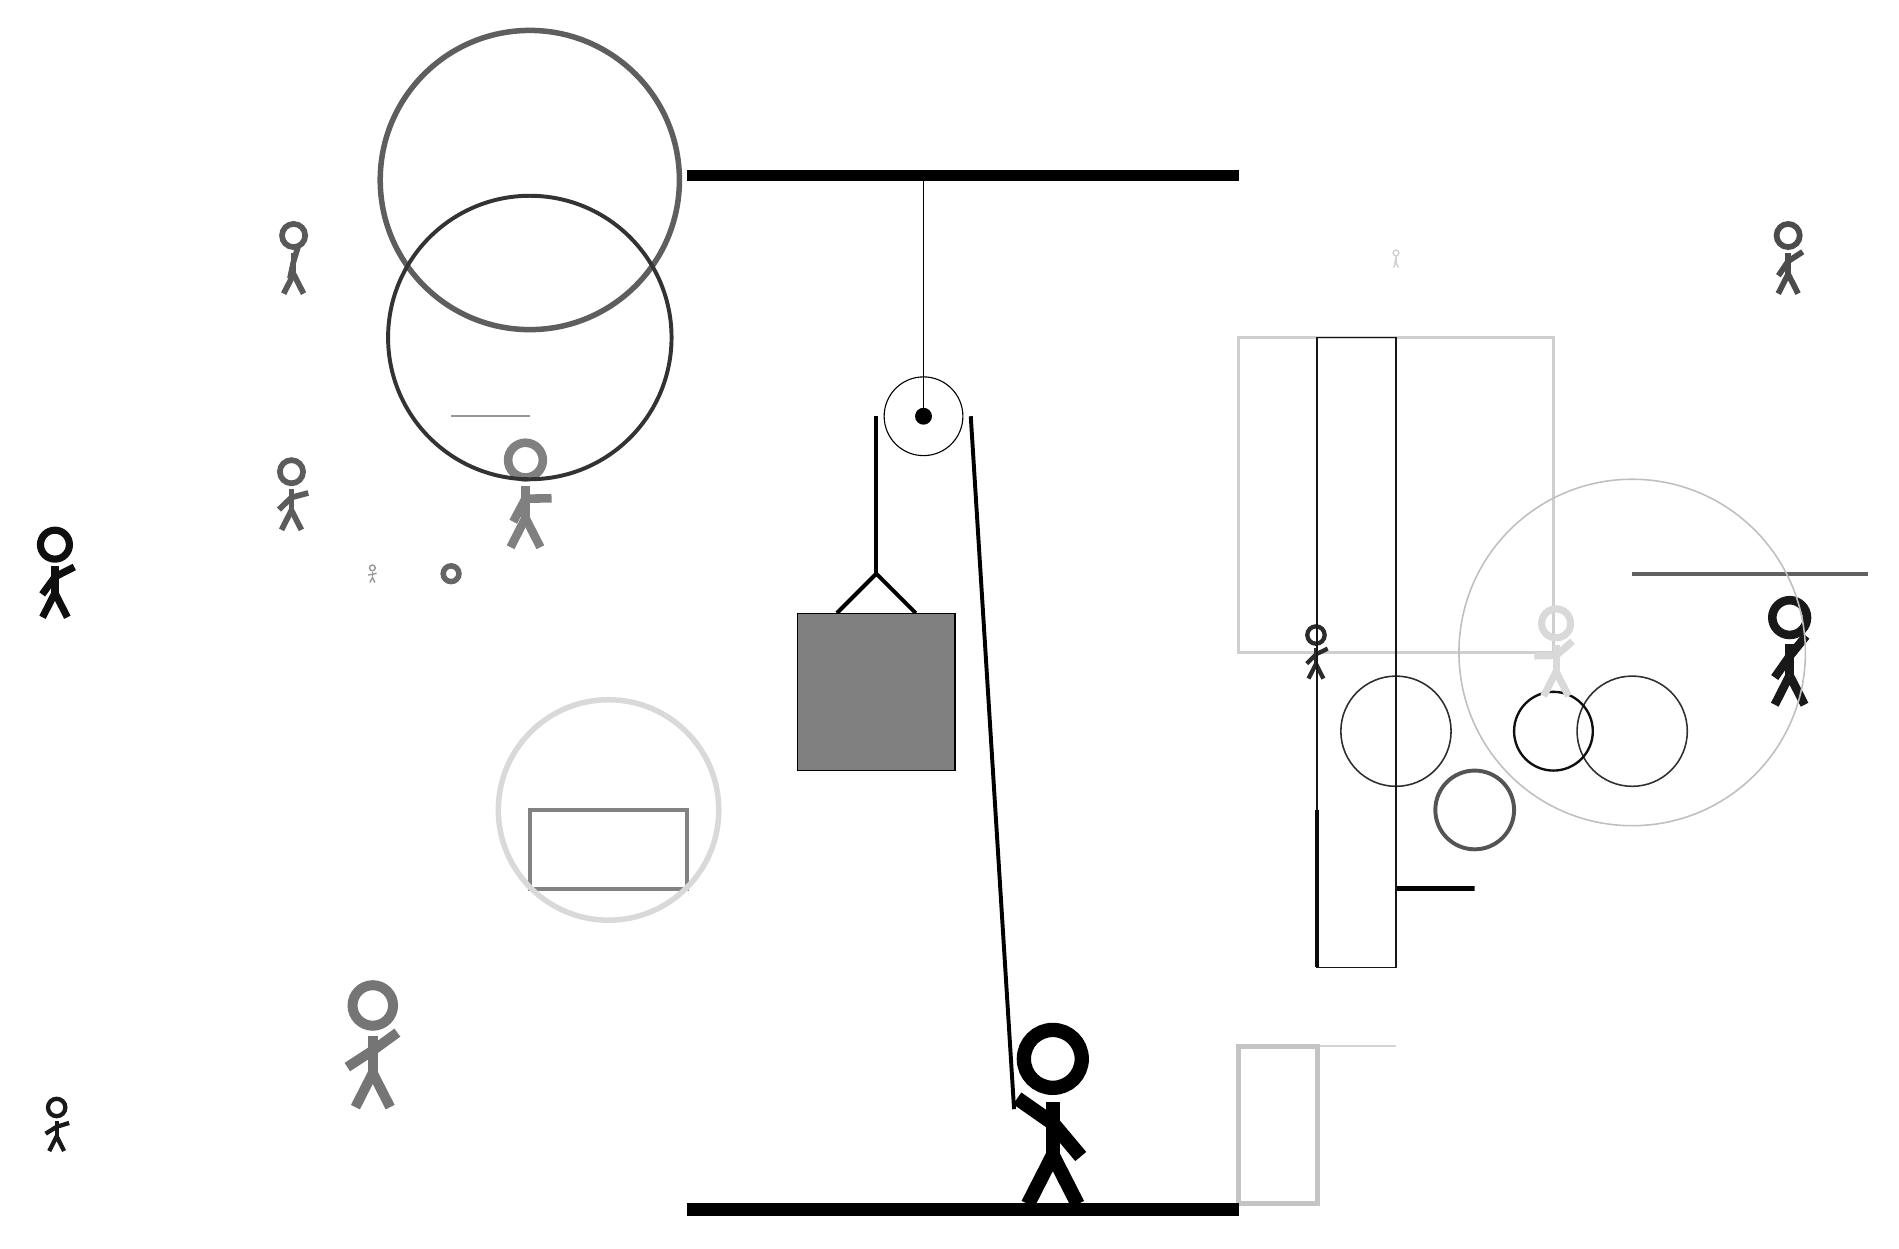
\begin{tikzpicture}
		%%%%% START %%%%%
		
		\draw[fill=black] (-2, 10) rectangle (5, 10.125);
		
		\node[line width=0.7mm, color=black!90] at (-10, -2) {\Strichmaxerl[3][32][17]};
		
		\draw [line width=0.2mm, color=black!82](7, 3) circle (0.7);
		\draw[line width=0.5mm, color=black!62](10, 5) -- (13, 5);
		\draw [line width=0.7mm, color=black!63](-4, 10) circle (1.9);
		
		\node[line width=0.4mm, color=black!64] at (-7, 6) {\Strichmaxerl[4][44][15]};
		\draw[line width=0.5mm, color=black!49] (-2, 1) rectangle (-4, 2);
		\draw[line width=0.3mm, color=black!17] (7, -1) rectangle (5, -1);
		\draw[line width=0.2mm, color=black!41] (-4, 7) rectangle (-5, 7);
		\draw [line width=0.7mm, color=black!60](-5, 5) circle (0.1);
		\draw[line width=0.7mm, color=black!99] (7, 1) rectangle (8, 1);
		\draw [line width=0.5mm, color=black!67](8, 2) circle (0.5);
		
		\node[line width=0.5mm, color=black!18] at (7, 9) {\Strichmaxerl[1][69][81]};
		\draw [line width=0.7mm, color=black!15](-3, 2) circle (1.4);
		
		\draw [line width=0.3mm, color=black!80](-3, -1) circle (0.0);
		\draw [line width=0.2mm, color=black!81](10, 3) circle (0.7);
		\draw [line width=0.3mm, color=black!94](9, 3) circle (0.5);
		
		\node[line width=0.6mm, color=black!50] at (-4, 6) {\Strichmaxerl[6][62][1]};
		\node[line width=0.5mm, color=black!40] at (-6, 5) {\Strichmaxerl[1][9][16]};
		\node[line width=0.2mm, color=black!90] at (12, 4) {\Strichmaxerl[6][55][51]};
		\draw[line width=0.4mm, color=black!19] (5, 8) rectangle (9, 4);
		\node[line width=0.7mm, color=black!94] at (-10, 5) {\Strichmaxerl[5][54][27]};
		
		\node[line width=0.3mm, color=black!83] at (6, 4) {\Strichmaxerl[3][45][26]};
		\node[line width=0.5mm, color=black!54] at (-6, -1) {\Strichmaxerl[7][33][36]};
		\node[line width=0.4mm, color=black!65] at (-7, 9) {\Strichmaxerl[4][78][73]};
		\draw [line width=0.2mm, color=black!25](10, 4) circle (2.2);
		
		\node[line width=0.7mm, color=black!70] at (12, 9) {\Strichmaxerl[4][56][33]};
		
		\node[line width=0.2mm, color=black!15] at (9, 4) {\Strichmaxerl[5][1][41]};
		\draw[line width=0.2mm, color=black!91] (7, 0) rectangle (6, 8);
		\draw [line width=0.5mm, color=black!80](-4, 8) circle (1.8);
		\draw[line width=0.5mm, color=black!96](6, 0) -- (6, 2);
		\draw[line width=0.6mm, color=black!23] (6, -3) rectangle (5, -1);
		
		\draw (1, 7) circle (0.5);
		\draw[fill=black] (1, 7) circle (0.1);
		\draw (1, 10) -- (1, 7);
		
		\draw[line width=0.5mm] (-0.1, 4.5) -- (0.4, 5.0) -- (0.9, 4.5);
		\draw[fill=black!50] (-0.6, 4.5) rectangle (1.4, 2.5);
		
		\draw[line width=0.5mm] (0.4, 7) -- (0.4, 5.0);
		\centerarc[line width=0.5mm](1, 7)(0:180:0.6);
		\draw[line width=0.5mm](1.6, 7) -- (2.15, -1.8);
		
		\node at (2.6, -1.9) {\Strichmaxerl[10][-35][-50]};
		
		\draw[fill=black] (-2, -3) rectangle (5, -3.15);
		
		%%%%% END %%%%%
	\end{tikzpicture}
\end{document}